%% abtex2-modelo-trabalho-academico.tex, v<VERSION> laurocesar
%% Copyright 2012-<COPYRIGHT_YEAR> by abnTeX2 group at http://www.abntex.net.br/ 
%%
%% This work may be distributed and/or modified under the
%% conditions of the LaTeX Project Public License, either version 1.3
%% of this license or (at your option) any later version.
%% The latest version of this license is in
%%   http://www.latex-project.org/lppl.txt
%% and version 1.3 or later is part of all distributions of LaTeX
%% version 2005/12/01 or later.
%%
%% This work has the LPPL maintenance status `maintained'.
%% 
%% The Current Maintainer of this work is the abnTeX2 team, led
%% by Lauro César Araujo. Further information are available on 
%% http://www.abntex.net.br/
%%
%% This work consists of the files abntex2-modelo-trabalho-academico.tex,
%% abntex2-modelo-include-comandos and abntex2-modelo-references.bib
%%

% ------------------------------------------------------------------------
% ------------------------------------------------------------------------
% abnTeX2: Modelo de Trabalho Academico (tese de doutorado, dissertacao de
% mestrado e trabalhos monograficos em geral) em conformidade com 
% ABNT NBR 14724:2011: Informacao e documentacao - Trabalhos academicos -
% Apresentacao
% ------------------------------------------------------------------------
% ------------------------------------------------------------------------

\documentclass[
	% -- opções da classe memoir --
	12pt,				% tamanho da fonte
	openright,			% capítulos começam em pág ímpar (insere página vazia caso preciso)
	twoside,			% para impressão em recto e verso. Oposto a oneside
	a4paper,			% tamanho do papel. 
	% -- opções da classe abntex2 --
	%chapter=TITLE,		% títulos de capítulos convertidos em letras maiúsculas
	%section=TITLE,		% títulos de seções convertidos em letras maiúsculas
	%subsection=TITLE,	% títulos de subseções convertidos em letras maiúsculas
	%subsubsection=TITLE,% títulos de subsubseções convertidos em letras maiúsculas
	% -- opções do pacote babel --
	english,			% idioma adicional para hifenização
	french,				% idioma adicional para hifenização
	spanish,			% idioma adicional para hifenização
	brazil				% o último idioma é o principal do documento
	]{abntex2}

% ---
% Pacotes básicos 
% ---
\usepackage{lmodern}			% Usa a fonte Latin Modern			
\usepackage[T1]{fontenc}		% Selecao de codigos de fonte.
\usepackage[utf8]{inputenc}		% Codificacao do documento (conversão automática dos acentos)
\usepackage{indentfirst}		% Indenta o primeiro parágrafo de cada seção.
\usepackage{color}				% Controle das cores
\usepackage{graphicx}			% Inclusão de gráficos
\graphicspath{ {./Imagens/} }
\usepackage{microtype} 			% para melhorias de justificação
% ---
		
% ---
% Pacotes adicionais, usados apenas no âmbito do Modelo Canônico do abnteX2
% ---
\usepackage{lipsum}				% para geração de dummy text
% ---

% ---
% Pacotes de citações
% ---
\usepackage[brazilian,hyperpageref]{backref}	 % Paginas com as citações na bibl
\usepackage[alf]{abntex2cite}	% Citações padrão ABNT

% ---
% Pacotes adicionados por mim (além dos do modelo!)
% ---
\usepackage[autostyle=true]{csquotes}   %Pacote de quotations (aspas)
% \usepackage[table]{xcolor}
% ---

% --- 
% CONFIGURAÇÕES DE PACOTES
% --- 

% ---
% Configurações do pacote backref
% Usado sem a opção hyperpageref de backref
\renewcommand{\backrefpagesname}{Citado na(s) página(s):~}
% Texto padrão antes do número das páginas
\renewcommand{\backref}{}
% Define os textos da citação
\renewcommand*{\backrefalt}[4]{
	\ifcase #1 %
		Nenhuma citação no texto.%
	\or
		Citado na página #2.%
	\else
		Citado #1 vezes nas páginas #2.%
	\fi}%
% ---

% ---
% Informações de dados para CAPA e FOLHA DE ROSTO
% ---
\titulo{Paralelização de Algoritmos Notórios de\\ Clustering em GPUs NVIDIA}
\autor{Vinícius Henrique Almeida Praxedes}
\local{Brasil}
\data{2019, Novembro}
\orientador{Daniel Duarte Abdala}
%\coorientador{Equipe \abnTeX}
\instituicao{%
  Universidade Federal de Uberlândia -- UFU
  \par
  Faculdade de Computação
  \par
  Programa de Graduação}
\tipotrabalho{Monografia}
% O preambulo deve conter o tipo do trabalho, o objetivo, 
% o nome da instituição e a área de concentração 
\preambulo{Monografia acadêmica apresentada à Faculdade de Computação da Universidade Federal de Uberlândia como parte dos requisitos necessários à obtenção do diploma do curso de Ciência da Computação}
% ---


% ---
% Configurações de aparência do PDF final

% alterando o aspecto da cor azul
\definecolor{blue}{RGB}{41,5,195}

% informações do PDF
\makeatletter
\hypersetup{
     	%pagebackref=true,
		pdftitle={\@title}, 
		pdfauthor={\@author},
    	pdfsubject={\imprimirpreambulo},
	    pdfcreator={LaTeX with abnTeX2},
		pdfkeywords={abnt}{latex}{abntex}{abntex2}{trabalho acadêmico}, 
		colorlinks=true,       		% false: boxed links; true: colored links
    	linkcolor=blue,          	% color of internal links
    	citecolor=blue,        		% color of links to bibliography
    	filecolor=magenta,      		% color of file links
		urlcolor=blue,
		bookmarksdepth=4
}
\makeatother
% --- 

% ---
% Posiciona figuras e tabelas no topo da página quando adicionadas sozinhas
% em um página em branco. Ver https://github.com/abntex/abntex2/issues/170
\makeatletter
\setlength{\@fptop}{5pt} % Set distance from top of page to first float
\makeatother
% ---

% ---
% Possibilita criação de Quadros e Lista de quadros.
% Ver https://github.com/abntex/abntex2/issues/176
%
\newcommand{\quadroname}{Quadro}
\newcommand{\listofquadrosname}{Lista de quadros}

\newfloat[chapter]{quadro}{loq}{\quadroname}
\newlistof{listofquadros}{loq}{\listofquadrosname}
\newlistentry{quadro}{loq}{0}

% configurações para atender às regras da ABNT
\setfloatadjustment{quadro}{\centering}
\counterwithout{quadro}{chapter}
\renewcommand{\cftquadroname}{\quadroname\space} 
\renewcommand*{\cftquadroaftersnum}{\hfill--\hfill}

\setfloatlocations{quadro}{hbtp} % Ver https://github.com/abntex/abntex2/issues/176
% ---

% --- 
% Espaçamentos entre linhas e parágrafos 
% --- 

% O tamanho do parágrafo é dado por:
\setlength{\parindent}{1.3cm}

% Controle do espaçamento entre um parágrafo e outro:
\setlength{\parskip}{0.2cm}  % tente também \onelineskip

% ---
% compila o indice
% ---
\makeindex
% ---

% ----
% Variáveis e definições
\def\qntAlgrtm{quatro}
\def\qntAlgrtmNaoExtenso{4}
% ----

% ----
% Início do documento
% ----
\begin{document}

% Seleciona o idioma do documento (conforme pacotes do babel)
%\selectlanguage{english}
\selectlanguage{brazil}

% Retira espaço extra obsoleto entre as frases.
\frenchspacing 

% ----------------------------------------------------------
% ELEMENTOS PRÉ-TEXTUAIS
% ----------------------------------------------------------
% \pretextual

% ---
% Capa
% ---
\imprimircapa
% ---

% ---
% Folha de rosto
% (o * indica que haverá a ficha bibliográfica)
% ---
\imprimirfolhaderosto*
% ---

% ---
% Inserir a ficha bibliografica
% ---

% Isto é um exemplo de Ficha Catalográfica, ou ``Dados internacionais de
% catalogação-na-publicação''. Você pode utilizar este modelo como referência. 
% Porém, provavelmente a biblioteca da sua universidade lhe fornecerá um PDF
% com a ficha catalográfica definitiva após a defesa do trabalho. Quando estiver
% com o documento, salve-o como PDF no diretório do seu projeto e substitua todo
% o conteúdo de implementação deste arquivo pelo comando abaixo:
%
% \begin{fichacatalografica}
%     \includepdf{fig_ficha_catalografica.pdf}
% \end{fichacatalografica}

\begin{fichacatalografica}
	\sffamily
	\vspace*{\fill}					% Posição vertical
	\begin{center}					% Minipage Centralizado
	\fbox{\begin{minipage}[c][8cm]{13.5cm}		% Largura
	\small
	\imprimirautor
	%Sobrenome, Nome do autor
	
	\hspace{0.5cm} \imprimirtitulo  / \imprimirautor. --
	\imprimirlocal, \imprimirdata-
	
	\hspace{0.5cm} \thelastpage p. : il. (algumas color.) ; 30 cm.\\
	
	\hspace{0.5cm} \imprimirorientadorRotulo~\imprimirorientador\\
	
	\hspace{0.5cm}
	\parbox[t]{\textwidth}{\imprimirtipotrabalho~--~\imprimirinstituicao,
	\imprimirdata.}\\
	
	\hspace{0.5cm}
		1. Palavra-chave1.
		2. Palavra-chave2.
		2. Palavra-chave3.
		I. Orientador.
		II. Universidade Federal de Uberlândia.
		III. Faculdade de Computação.
		IV. Título 			
	\end{minipage}}
	\end{center}
\end{fichacatalografica}
% ---

% ---
% Inserir errata
% ---
% \begin{errata}
% Elemento opcional da \citeonline[4.2.1.2]{NBR14724:2011}. Exemplo:

% \vspace{\onelineskip}

% FERRIGNO, C. R. A. \textbf{Tratamento de neoplasias ósseas apendiculares com
% reimplantação de enxerto ósseo autólogo autoclavado associado ao plasma
% rico em plaquetas}: estudo crítico na cirurgia de preservação de membro em
% cães. 2011. 128 f. Tese (Livre-Docência) - Faculdade de Medicina Veterinária e
% Zootecnia, Universidade de São Paulo, São Paulo, 2011.

% \begin{table}[htb]
% \center
% \footnotesize
% \begin{tabular}{|p{1.4cm}|p{1cm}|p{3cm}|p{3cm}|}
%   \hline
%   \textbf{Folha} & \textbf{Linha}  & \textbf{Onde se lê}  & \textbf{Leia-se}  \\
%     \hline
%     1 & 10 & auto-conclavo & autoconclavo\\
%   \hline
% \end{tabular}
% \end{table}

% \end{errata}
% ---

% ---
% Inserir folha de aprovação
% ---

% Isto é um exemplo de Folha de aprovação, elemento obrigatório da NBR
% 14724/2011 (seção 4.2.1.3). Você pode utilizar este modelo até a aprovação
% do trabalho. Após isso, substitua todo o conteúdo deste arquivo por uma
% imagem da página assinada pela banca com o comando abaixo:
%
% \begin{folhadeaprovacao}
% \includepdf{folhadeaprovacao_final.pdf}
% \end{folhadeaprovacao}
%
\begin{folhadeaprovacao}

  \begin{center}
    {\ABNTEXchapterfont\large\imprimirautor}

    \vspace*{\fill}\vspace*{\fill}
    \begin{center}
      \ABNTEXchapterfont\bfseries\Large\imprimirtitulo
    \end{center}
    \vspace*{\fill}
    
    \hspace{.45\textwidth}
    \begin{minipage}{.5\textwidth}
        \imprimirpreambulo
    \end{minipage}%
    \vspace*{\fill}
   \end{center}
        
   Trabalho aprovado. \imprimirlocal, 24 de novembro de 2012:

   \assinatura{\textbf{\imprimirorientador} \\ Orientador} 
   \assinatura{\textbf{Professor} \\ Convidado 1}
   \assinatura{\textbf{Professor} \\ Convidado 2}
   %\assinatura{\textbf{Professor} \\ Convidado 3}
   %\assinatura{\textbf{Professor} \\ Convidado 4}
      
   \begin{center}
    \vspace*{0.5cm}
    {\large\imprimirlocal}
    \par
    {\large\imprimirdata}
    \vspace*{1cm}
  \end{center}
  
\end{folhadeaprovacao}
% ---

% % ---
% % Dedicatória
% % ---
% \begin{dedicatoria}
%   \vspace*{\fill}
%   \centering
%   \noindent
%   \textit{ Este trabalho é dedicado às crianças adultas que,\\
%   quando pequenas, sonharam em se tornar cientistas.} \vspace*{\fill}
% \end{dedicatoria}
% % ---

% % ---
% % Agradecimentos
% % ---
% \begin{agradecimentos}
% Os agradecimentos principais são direcionados à Gerald Weber, Miguel Frasson,
% Leslie H. Watter, Bruno Parente Lima, Flávio de Vasconcellos Corrêa, Otavio Real
% Salvador, Renato Machnievscz\footnote{Os nomes dos integrantes do primeiro
% projeto abn\TeX\ foram extraídos de
% \url{http://codigolivre.org.br/projects/abntex/}} e todos aqueles que
% contribuíram para que a produção de trabalhos acadêmicos conforme
% as normas ABNT com \LaTeX\ fosse possível.

% Agradecimentos especiais são direcionados ao Centro de Pesquisa em Arquitetura
% da Informação\footnote{\url{http://www.cpai.unb.br/}} da Universidade de
% Brasília (CPAI), ao grupo de usuários
% \emph{latex-br}\footnote{\url{http://groups.google.com/group/latex-br}} e aos
% novos voluntários do grupo
% \emph{\abnTeX}\footnote{\url{http://groups.google.com/group/abntex2} e
% \url{http://www.abntex.net.br/}}~que contribuíram e que ainda
% contribuirão para a evolução do \abnTeX.

% \end{agradecimentos}
% % ---

% % ---
% % Epígrafe
% % ---
% \begin{epigrafe}
%     \vspace*{\fill}
% 	\begin{flushright}
% 		\textit{``Não vos amoldeis às estruturas deste mundo, \\
% 		mas transformai-vos pela renovação da mente, \\
% 		a fim de distinguir qual é a vontade de Deus: \\
% 		o que é bom, o que Lhe é agradável, o que é perfeito.\\
% 		(Bíblia Sagrada, Romanos 12, 2)}
% 	\end{flushright}
% \end{epigrafe}
% % ---

% % ---
% % RESUMOS
% % ---

% % resumo em português
% \setlength{\absparsep}{18pt} % ajusta o espaçamento dos parágrafos do resumo
% \begin{resumo}
%  Segundo a \citeonline[3.1-3.2]{NBR6028:2003}, o resumo deve ressaltar o
%  objetivo, o método, os resultados e as conclusões do documento. A ordem e a extensão
%  destes itens dependem do tipo de resumo (informativo ou indicativo) e do
%  tratamento que cada item recebe no documento original. O resumo deve ser
%  precedido da referência do documento, com exceção do resumo inserido no
%  próprio documento. (\ldots) As palavras-chave devem figurar logo abaixo do
%  resumo, antecedidas da expressão Palavras-chave:, separadas entre si por
%  ponto e finalizadas também por ponto.

%  \textbf{Palavras-chave}: latex. abntex. editoração de texto.
% \end{resumo}

% % resumo em inglês
% \begin{resumo}[Abstract]
%  \begin{otherlanguage*}{english}
%   This is the english abstract.

%   \vspace{\onelineskip}
 
%   \noindent 
%   \textbf{Keywords}: latex. abntex. text editoration.
%  \end{otherlanguage*}
% \end{resumo}

% % resumo em francês 
% \begin{resumo}[Résumé]
%  \begin{otherlanguage*}{french}
%     Il s'agit d'un résumé en français.
 
%   \textbf{Mots-clés}: latex. abntex. publication de textes.
%  \end{otherlanguage*}
% \end{resumo}

% % resumo em espanhol
% \begin{resumo}[Resumen]
%  \begin{otherlanguage*}{spanish}
%   Este es el resumen en español.
  
%   \textbf{Palabras clave}: latex. abntex. publicación de textos.
%  \end{otherlanguage*}
% \end{resumo}
% % ---

% % ---
% % inserir lista de ilustrações
% % ---
% \pdfbookmark[0]{\listfigurename}{lof}
% \listoffigures*
% \cleardoublepage
% % ---

% % ---
% % inserir lista de quadros
% % ---
% \pdfbookmark[0]{\listofquadrosname}{loq}
% \listofquadros*
% \cleardoublepage
% % ---

% % ---
% % inserir lista de tabelas
% % ---
% \pdfbookmark[0]{\listtablename}{lot}
% \listoftables*
% \cleardoublepage
% % ---

% % ---
% % inserir lista de abreviaturas e siglas
% % ---
% \begin{siglas}
%   \item[ABNT] Associação Brasileira de Normas Técnicas
%   \item[abnTeX] ABsurdas Normas para TeX
% \end{siglas}
% % ---

% % ---
% % inserir lista de símbolos
% % ---
% \begin{simbolos}
%   \item[$ \Gamma $] Letra grega Gama
%   \item[$ \Lambda $] Lambda
%   \item[$ \zeta $] Letra grega minúscula zeta
%   \item[$ \in $] Pertence
% \end{simbolos}
% % ---

% ---
% inserir o sumario
% ---
\pdfbookmark[0]{\contentsname}{toc}
\tableofcontents*
\cleardoublepage
% ---



% ----------------------------------------------------------
% ELEMENTOS TEXTUAIS
% ----------------------------------------------------------
\textual

% ----------------------------------------------------------
% Capítulo - Introdução
% ----------------------------------------------------------
\chapter{Introdução}
% ----------------------------------------------------------

A busca pelo menor tempo de execução é uma diretriz ubíqua na computação. Desde os primórdios da área buscamos algoritmos e procedimentos que, dados os mesmos parâmetros de entrada, executem a mesma tarefa na menor quantidade de tempo possível. Outros recursos como espaço de memória utilizado, eficiência energética ou uso da rede em muitos cenários são mais importantes que o tempo de execução, mas ainda sim a mesma continua sendo um dos mais estudados parâmetros para categorização e avaliação de algoritmos e procedimentos na computação. De fato o tempo de execução -- em ciclos, ou passos, de processamento -- é a métrica utilizada na análise de uma das maiores incógnitas da computação, o problema P versus NP.

Um grande avanço na quantidade de poder de processamento dos computadores e, portanto, diminuição do tempo de execução de algoritmos, foi a paralelização dos processadores. A habilidade de poder executar duas ou mais ações simultaneamente possibilitou muitos ganhos palpáveis na velocidade de execução de algoritmos e procedimentos, porém introduziu uma necessidade de mudança na forma de se pensar em resoluções de problemas computacionalmente: paralelizar um algoritmo antes serial não é uma tarefa trivial, e requer cuidados especiais com concorrência no acesso a recursos da máquina, dependência de dados e cálculos, sincronização, entre outros dilemas.

Um dos componentes que mais utilizam da paralelização num computador moderno são as GPUs, unidades de processamento gráfico, ou placas de vídeo, que são basicamente processadores especializados em operações vetoriais, altamente paralelizadas, usualmente dedicados a operações gráficas, e com sua própria memória dedicada, a VRAM. Enquanto processadores de uso geral, CPUs, costumam ter no máximo dezenas de núcleos para processamento paralelo, GPUs possuem milhares ou até milhões de núcleos para operações vetoriais.

No entanto, cada vez mais está sendo descoberto e aproveitado o potencial de uso das GPUs em atividades não apenas voltadas para renderização, interfaces e outras operações gráficas, mas para a computação de propósito geral. Diversos algoritmos modernos e antigos beneficiam-se imensamente da paralelização enorme proporcionada por GPUs, e com ferramentas como a biblioteca e linguagem CUDA criada pela NVIDIA, está cada vez mais fácil implementar o uso de placas de vídeo em conjunto com CPUs convencionais nos mais variados algoritmos.

Nem todo algoritmo pode ser paralelizado, no entanto. Existem procedimentos e algoritmos que são inerentemente seriais, como o cálculo do $n$-ésimo número da sequência de \textit{Fibonacci}, que requer que dois números prévios da sequência tenham sido calculados para obtermos o atual -- salvo, é claro, alguma descoberta teórica matemática do comportamento da sequência que nos permitisse uma nova maneira de calcular o $n$-ésimo elemento sem essa necessidade.

É importante entender também que nenhum algoritmo é paralelizável por completo. Sempre existem partes de algoritmos que devem ser executadas serialmente para funcionar corretamente. O ganho máximo da paralelização de um algoritmo qualquer é uma função da parcela do seu código que pode ser paralelizada, e é definida pela Lei de Amdahl \cite{Amdahl-Law}: $\frac{1}{1-p}$, onde $p$ é a razão entre código paralelizável e código não-paralelizável.

E é a paralelização de uma classe de algoritmos em especial que é o foco desta pesquisa: algoritmos de \textit{clustering}, ou clusterização. Tais algoritmos, de forma sucinta, agrupam objetos de maneira que os objetos no mesmo grupo, ou \textit{cluster}, sejam mais parecidos entre si, de acordo com alguma métrica, do que com objetos de outros grupos. A análise de clusters é essencial em diversas áreas da computação, como mineração de dados, aprendizado de máquina, compressão de dados, entre outras.

% !!!!!!!!!!!!!!!!!!!!!!!!!!!!
% Checar se essa citação do site da NVIDIA está correta! Esse bagulho no Bib usou o modelo "misc", não sei se está correto. O Mendeley gerou assim, então talvez esteja...
% !!!!!!!!!!!!!!!!!!!!!!!!!!!!

A hipótese principal é a de que algoritmos de clustering, em geral, são altamente paralelizáveis, e apresentam um ganho considerável de desempenho (menor tempo de execução) quando implementados para utilizar o poder de paralelismo vetorial de placas de vídeo NVIDIA, através da linguagem CUDA \cite{CUDAZone}. Mais que isso, através de uma análise sistemática de estudos prévios e implementações de tais algoritmos em CUDA, visa-se generalizar o processo de paralelização destes. Isto é, identificar quais partes são necessariamente seriais, quais são paralelizáveis, e que sequência de passos gerais deve ser seguida para se conseguir paralelizar com sucesso e ganho significativo de desempenho um algoritmo de clustering qualquer.

% !!!!!!!!!!!!!!!!!!!!!!!!!!!!
% Tenho que substituir essas referências aqui por referências de versões seriais de cada algoritmo. Usar as referências das versões aceleradas em GPUs mais adiante, ao invés de aqui parece fazer bem mais sentido
% !!!!!!!!!!!!!!!!!!!!!!!!!!!!

O foco de pesquisa são \qntAlgrtm{} algoritmos de clustering especialmente notórios: \textit{K-means} \cite{GPU-accelerated-K-Means}, \textit{Clustering Hierárquico}, \textit{DBSCAN} \cite{G-DBSCAN}, ou \textit{Clusterização Espacial Baseada em Densidade de Aplicações com Ruído}, e \textit{Random Forests} -- que mesmo não sendo exclusivamente um algoritmo de clusterização, pode ser utilizado justamente para tal. Implementações e estudos realizados sobre estes serão analisados, e implementações novas terão desempenho comparado com estas.

% ----

\section{Objetivos}

\subsection{Objetivo Geral}

Esse trabalho tem como objetivo principal testar a validez de sua hipótese (discutida mais à fundo na seção 1.2) de que algoritmos de clusterização são intrinsecamente paralelizáveis, e que o ganho de velocidade ao serem paralelizados é altamente significativo.

Além disso, deseja-se compilar aqui um vasto conhecimento de como paralelizar esses algoritmos em geral, analisando principalmente os \qntAlgrtm{} aqui estudados a fundo (k-means, clustering hierárquico, DBSCAN e Random Forests) e usando este aprendizado para criar um passo-a-passo genérico de como realizar tal modificação de código em um algoritmo de clusterização qualquer.

\subsection{Objetivos Específicos}

Para atingir o objetivo geral, será necessário completar diversos objetivos menores, ou \textit{milestones}, antes, criando um caminho de pesquisa a ser seguido --- não necessariamente na ordem apresentada. São estes:

\begin{itemize}
    \item Pesquisar extensamente a bibliografia da área, realizando assim um levantamento do estado da arte de algoritmos paralelos de clusterização;
    \item Estudar implementações já realizadas dos \qntAlgrtm{} algoritmos aqui estudados, a fim de adquirir conhecimento de como a paralelização em CUDA deve ser realizada;
    % !!!!!!!!!!!!!!!!!!!!!!!!!!!!
    % Tenho que aprofundar nesse tópico, explicando qual algoritmo de clustering "novo" será paralelizado afinal, quando eu escolher um de fato!
    % !!!!!!!!!!!!!!!!!!!!!!!!!!!!
    \item Paralelizar um algoritmo de clustering \enquote{novo}, isto é, nunca antes paralelizado e exibido em trabalho científico, a fim de solidificar o conhecimento e prática de programação em CUDA;
    \item Quantificar o ganho de desempenho das implementações paralelas, realizando diversos experimentos de \textit{speedup};
    \item Comparar código monolítico (sem paralelização) com código paralelo dos \qntAlgrtm{} algoritmos analisados, extraindo assim um conhecimento de como paralelizar um algoritmo de clusterização genérico;
\end{itemize}

% ----

\section{Hipótese}

A hipótese que esta pesquisa procura testar é a de que algoritmos de clusterização em geral são inerentemente vetoriais e, consequentemente, se beneficiariam significativamente de arquiteturas de processamento vetoriais, como uma unidade de processamento gráfico, ou GPU.

Um problema ser vetorial diz respeito ao escopo de itens de dados relevantes ao problema. Grande parte dos problemas da computação são escalares, o que significa que eles lidam com itens de dados unitários, como por exemplo \textit{integers} ou \textit{floats}, um de cada vez. Já um problema vetorial lida com itens de dados que são conjuntos unidimensionais, chamados vetores, que são formados por vários itens unitários de dados agrupados.

Um algoritmo que tente resolver um problema vetorial terá desempenho maior quando executado num processador vetorial, isto é, um processador que possui um conjunto de instruções capaz de manipular vetores. Apesar de um algoritmo de um problema vetorial ainda puder ser implementado e executado com sucesso num processador escalar, o desempenho será menor pois os dados vetoriais do problema terão que ter seus elementos processados um a um pelo processador, já que ele não trabalha com vetores propriamente ditos em seu conjunto de instruções.

Grande parte do ganho de desempenho supracitado vem do paralelismo proporcionado pelos processadores vetoriais, como GPUs, ao manipular conjuntos maiores de dados de uma só vez, e em vários núcleos simultaneamente, além de economizar traduções de endereço de memória e operações de obtenção (\textit{fetch}) e decodificação (\textit{decode}) de instruções, pois haverá um número muito menor de instruções e endereços de memória quando os dados estão agrupados em vetores, que podem ser manipulados e usados em operações como se fossem apenas um item de dados.

Este trabalho, então, visa demonstrar que algoritmos de clusterização, em geral, são intrinsecamente vetoriais. Isto é, qualquer algoritmo de clustering concebível será de natureza vetorial, pois estes analisam dados e tentam agrupá-los de a acordo com algum grau de semelhança entre eles, análise essa que pode ser feita com conjuntos dos itens de dados (vetores), ao invés de individualmente. Logo, qualquer algoritmo de clusterização teria uma parcela de seu código que seria paralelizável, e assim ganhariam desempenho significativo com uma execução numa GPU.

% ----

\section{Justificativa}

A pesquisa feita aqui pode ser de grande utilidade para a área de análise de clusters, e impulsionar a implementação de mais algoritmos paralelos de clusterização.

Com a compilação de conhecimento realizada aqui a intenção é facilitar pesquisas posteriores na área de paralelização de algoritmos de clustering e motivar novas implementações paralelas de outros algoritmos dessa classe com os experimentos de ganho de desempenho, ilustrando o quão importante é o uso de processadores vetoriais como GPUs para tornar o uso de alguns destes algoritmos prático.

Além disso, a apresentação nesse estudo de um procedimento genérico para paralelizar qualquer algoritmo de clustering será de extrema utilidade para qualquer desenvolvedor ou pesquisador que desejar implementar uma versão acelerada em GPU de um algoritmo de clusterização, mesmo este sendo totalmente novo. No mínimo servirá de ponto de partida para o entendimento e aprendizado de como realizar tal modificação no código do algoritmo, e renderá uma implementação que serve de base para estudos e otimizações, até se atingir uma implementação digna para uso prático.

% ----------------------------------------------------------
% Capítulo - Fundamentação Teórica
% ----------------------------------------------------------

\chapter{Fundamentação Teórica}

Para compreender a pesquisa científica aqui realizada, é necessário primeiro entender o que são algoritmos de clusterização, tanto de maneira geral quanto específica, explorando os fundamentos e funcionamento dos \qntAlgrtm{} algoritmos pesquisados. Veremos que a complexidade de tempo destes algoritmos tendem a ser inconvenientemente altas ($O(n\cdot\log{n})$, $O(n^2)$ ou até $O(n^3)$ sendo complexidades comuns) e por isso qualquer ganho de velocidade significativo obtido valerá muito a pena.

Também é imprescindível explorar o funcionamento dos processadores vetoriais --- sendo as \textit{Unidades de Processamento Gráfico} (GPUs) o principal exemplo destes e sobre o qual essa pesquisa irá focar --- e entender por quê usá-los para paralelizar algoritmos de clusterização proporcionará, em tese, um ganho de velocidade expressivo na execução destes, abrandando o peso de suas complexidades de tempo. Além de tudo isso, será apresentada brevemente a arquitetura que será utilizada para paralelizar os algoritmos estudados: a plataforma e modelo de programação CUDA, da NVIDIA, que permitirá extrair o poder de paralelização das placas de vídeo NVIDIA.

% ----

\section{Clusterização}

A clusterização, ou clustering, é a tarefa de agrupar um conjunto de elementos de modo que cada elemento de um grupo se \enquote{pareça} mais com outros elementos do grupo (cluster) que pertence do que com elementos dos grupos que não pertence --- para algum significado bem definido de semelhança. É um processo muito comum e virtualmente necessário nas áreas de mineração de dados, análise estatística, análise de imagem, aprendizado de máquina, reconhecimento de padrões, e muitas outras.

O significado de um cluster não pode ser bem definido e vai depender do conjunto de dados a ser analisado e a forma que os resultados obtidos serão utilizados --- de fato, esse é o principal motivo pelo qual tantos algoritmos diferentes de clustering existem \cite{SoManyClustAlg}. O comum em todas definições usadas é que um cluster é um conjunto de objetos de dados. Esses objetos são representados num espaço de dimensões iguais ao número de dados relevantes para cada objeto, e os algoritmos tentam criar grupos (clusters) nesse espaço que agrupem os objetos de uma maneira significativa, ou útil, para o estudo sendo feito e a definição de cluster sendo utilizada.

% !!!!!!!!!!!!!!!!!!!!!!!!!!!!
% Talvez seria melhor colocar esse parágrafo num formato de lista? Não sei...
% Também não sei se meu uso do negrito aqui é permitido formalmente.
% !!!!!!!!!!!!!!!!!!!!!!!!!!!!

Diversos modelos de cluster podem ser usados para definir o que é um cluster: \textbf{modelos de centroide}, onde cada cluster possui um centro e os objetos pertencerão aos clusters com centros mais próximos deles, dada uma definição de distância no espaço de dados; \textbf{modelos de densidade}, que definem clusters como regiões densas e conexas no espaço de dados, contrastando com regiões menos densas que separam os clusters; \textbf{modelos de conectividade}, que constroem clusters a partir de conexões de objetos por distância; \textbf{modelos de distribuição}, que utilizam de distribuições estatísticas, como a distribuição normal ou exponencial, para modelar agrupamentos dos objetos; entre dezenas de outros modelos. Entender o modelo de cluster utilizado é essencial para compreender um algoritmo de clusterização e as diferenças entre a multitude destes.

% !!!!!!!!!!!!!!!!!!!!!!!!!!!!
% Eu preciso realmente ficar colocando termos em inglês não traduzidos (intraduzíveis de maneira sã, na maioria das vezes) em itálico? Isso me parece bem brega.
% !!!!!!!!!!!!!!!!!!!!!!!!!!!!

O resultado, ou saída, de um algoritmo de clusterização é comumente um rotulamento dos objetos de dados passados na entrada, o que indicará a divisão em clusters feita por ele. Classificações podem ser feitas quanto à natureza da clusterização obtida pelos algoritmos: \textbf{\textit{hard clustering}}, onde cada objeto pertence ou não a um cluster; \textbf{\textit{fuzzy clustering}}, onde cada objeto pertence uma certa porcentagem a cada cluster, o que pode significar, por exemplo, a chance do objeto pertencer àquele cluster \cite{FuzzyClusteringSurvey}. E subclassificações mais granulares ainda podem ser definidas, como: \textbf{clusterização de particionamento estrito}, onde cada objeto pertence a exatamente um cluster; \textbf{clusterização de particionamento estrito com \textit{outliers}}, onde objetos pertencem a exatamente um cluster, ou nenhum cluster, assim sendo considerados \textit{outliers}.

% \subsection{K-Means}

% \subsection{Clusterização Hierárquica}

% \subsection{DBSCAN}

% \subsection{Random Forests}

% ----

% \section{Processadores Vetoriais}

% \subsection{A Arquitetura NVIDIA / CUDA}

% \subsection{Como Programar em CUDA: Um Overview}

% ----

% \chapter{Levantamento do Estado da Arte}

% ----------------------------------------------------------
% Capítulo - Metodologia de Desenvolvimento e Pesquisa
% ----------------------------------------------------------

\chapter{Metodologia de Desenvolvimento e Pesquisa}

A pesquisa realizada neste trabalho consiste de estudos e análises de trabalhos prévios, desenvolvimento de uma versão paralelizada de um algoritmo de clustering e experimentos sobre essa implementação. Pode-se dividir tal metodologia em um conjunto de etapas.

A primeira etapa consiste de uma extensa pesquisa bibliográfica. O intuito é levantar o estado da arte na área de algoritmos de clusterização acelerados em GPU usando a linguagem e livraria CUDA da NVIDIA. Entender quais algoritmos já foram implementados com sucesso em CUDA, e como foi feita tal implementação, além dos resultados (ganhos em desempenho) das mesmas. Essa etapa agregará conhecimento sobre como utilizar CUDA para acelerar algoritmos de clustering, além de dar uma ideia do tipo de ganho de desempenho esperado de uma paralelização média desse tipo de algoritmo.

A segunda etapa consiste da implementação de uma versão paralela \enquote{inédita} de algum algum algoritmo de clusterização, ou seja, paralelizar um algoritmo nunca antes paralelizado e exibido em alguma pesquisa. Usando o aprendizado adquirido na primeira etapa de pesquisa, um algoritmo será paralelizado em CUDA, e seus resultados comparados com os resultados da versão serial (rodando somente numa CPU) para garantir corretude. Os ganhos de velocidade da versão acelerada em CUDA será então comparada também com os ganhos obtidos nos trabalhos analisados na primeira etapa. Isso servirá como uma medição da efetividade da implementação feita.

A terceira etapa consiste da busca de um procedimento geral para paralelizar um algoritmo de clustering genérico. Ou seja, encontrar um passo-a-passo de modificações ao código de um algoritmo serial que, ao fim, o transforme numa versão acelerada usando CUDA desse mesmo algoritmo, ainda mantendo sua corretude e proporcionando algum ganho de desempenho.

A quarta etapa, por fim, se trata de diversos experimentos de ganho de velocidade, ou \textit{speedup}, do algoritmo que teve aqui sua versão acelerada em GPU implementada e apresentada. Esses experimentos irão dar uma ideia do quão significativo foi o ganho de desempenho ao paralelizar o algoritmo usando CUDA, se há um teto ou chão para tais ganhos, como o \textit{speedup} aumenta ou diminui com o aumento do dataset a ser analisado, assim como realizar uma análise de outros parâmetros importantes que não sejam velocidade, como uso de memória --- afinal, as VRAMs das placas de vídeo são comumente mais limitadas em tamanho que as RAMs utilizadas pelas CPUs.

% \chapter{Experimentos e Datasets}

% \chapter{Conclusões}

% ----------------------------------------------------------
% Capítulo - Cronograma
% ----------------------------------------------------------

\chapter{Cronograma}

A tabela abaixo representa o cronograma de pesquisa e desenvolvimento deste trabalho. Cada célula da mesma representa uma semana de tempo (sete dias corridos), considerando cada mês como tendo exatamente quatro semanas. O período coberto vai de dezembro de 2019 à julho de 2020, data estimada de término da conclusão desta monografia.

\begin{figure}[h]
    \centering
    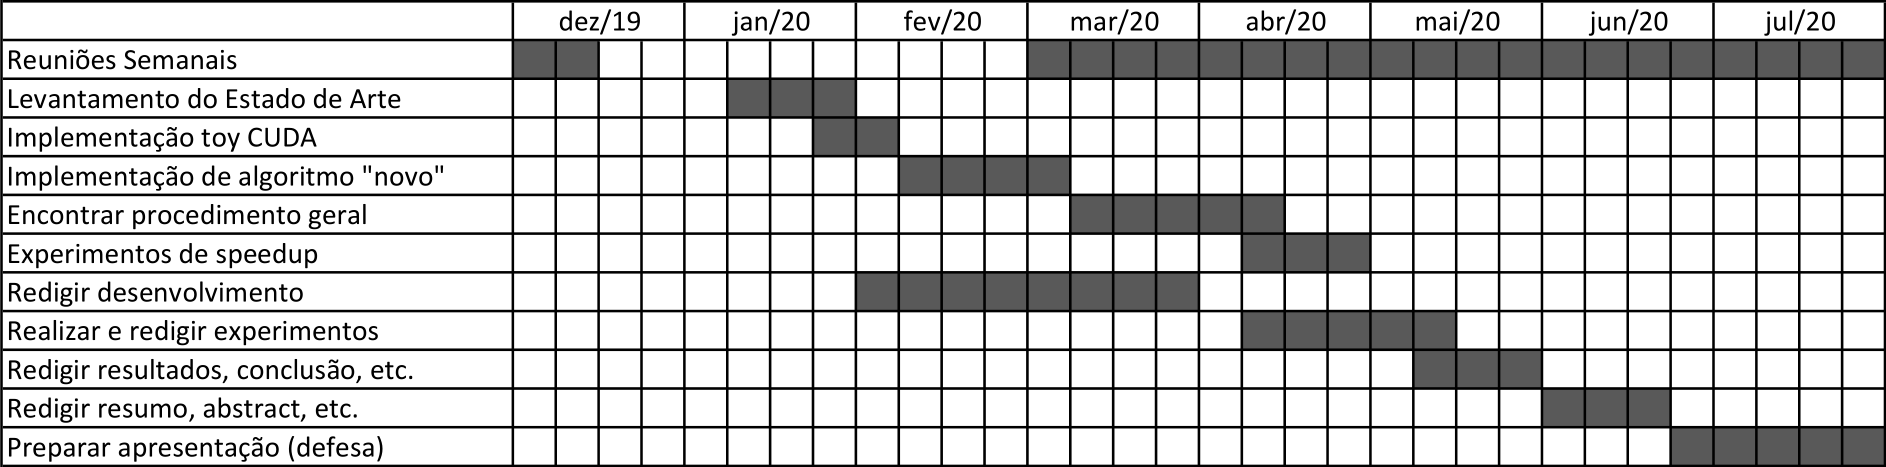
\includegraphics[width=\textwidth]{Cronograma_2-0}
    \caption{Cronograma de pesquisa e desenvolvimento}
    % \label{fig:my_label}
\end{figure}

% ----------------------------------------------------------

% % ----------------------------------------------------------
% % PARTE
% % ----------------------------------------------------------
% %\part{Preparação da pesquisa}
% % ----------------------------------------------------------

% % ---
% % Capitulo com exemplos de comandos inseridos de arquivo externo 
% % ---
% %% abtex2-modelo-include-comandos.tex, v<VERSION> laurocesar
%% Copyright 2012-<COPYRIGHT_YEAR> by abnTeX2 group at http://www.abntex.net.br/ 
%%
%% This work may be distributed and/or modified under the
%% conditions of the LaTeX Project Public License, either version 1.3
%% of this license or (at your option) any later version.
%% The latest version of this license is in
%%   http://www.latex-project.org/lppl.txt
%% and version 1.3 or later is part of all distributions of LaTeX
%% version 2005/12/01 or later.
%%
%% This work has the LPPL maintenance status `maintained'.
%% 
%% The Current Maintainer of this work is the abnTeX2 team, led
%% by Lauro César Araujo. Further information are available on 
%% http://www.abntex.net.br/
%%
%% This work consists of the files abntex2-modelo-include-comandos.tex
%% and abntex2-modelo-img-marca.pdf
%%

% ---
% Este capítulo, utilizado por diferentes exemplos do abnTeX2, ilustra o uso de
% comandos do abnTeX2 e de LaTeX.
% ---
 
\chapter{Resultados de comandos}\label{cap_exemplos}

\chapterprecis{Isto é uma sinopse de capítulo. A ABNT não traz nenhuma
normatização a respeito desse tipo de resumo, que é mais comum em romances 
e livros técnicos.}\index{sinopse de capítulo}

% ---
\section{Codificação dos arquivos: UTF8}
% ---

A codificação de todos os arquivos do \abnTeX\ é \texttt{UTF8}. É necessário que
você utilize a mesma codificação nos documentos que escrever, inclusive nos
arquivos de base bibliográficas |.bib|.

% ---
\section{Citações diretas}
\label{sec-citacao}
% ---

\index{citações!diretas}Utilize o ambiente \texttt{citacao} para incluir
citações diretas com mais de três linhas:

\begin{citacao}
As citações diretas, no texto, com mais de três linhas, devem ser
destacadas com recuo de 4 cm da margem esquerda, com letra menor que a do texto
utilizado e sem as aspas. No caso de documentos datilografados, deve-se
observar apenas o recuo \cite[5.3]{NBR10520:2002}.
\end{citacao}

Use o ambiente assim:

\begin{verbatim}
\begin{citacao}
As citações diretas, no texto, com mais de três linhas [...] deve-se observar
apenas o recuo \cite[5.3]{NBR10520:2002}.
\end{citacao}
\end{verbatim}

O ambiente \texttt{citacao} pode receber como parâmetro opcional um nome de
idioma previamente carregado nas opções da classe (\autoref{sec-hifenizacao}). Nesse
caso, o texto da citação é automaticamente escrito em itálico e a hifenização é
ajustada para o idioma selecionado na opção do ambiente. Por exemplo:

\begin{verbatim}
\begin{citacao}[english]
Text in English language in italic with correct hyphenation.
\end{citacao}
\end{verbatim}

Tem como resultado:

\begin{citacao}[english]
Text in English language in italic with correct hyphenation.
\end{citacao}

\index{citações!simples}Citações simples, com até três linhas, devem ser
incluídas com aspas. Observe que em \LaTeX as aspas iniciais são diferentes das
finais: ``Amor é fogo que arde sem se ver''.

% ---
\section{Notas de rodapé}
% ---

As notas de rodapé são detalhadas pela NBR 14724:2011 na seção 5.2.1\footnote{As
notas devem ser digitadas ou datilografadas dentro das margens, ficando
separadas do texto por um espaço simples de entre as linhas e por filete de 5
cm, a partir da margem esquerda. Devem ser alinhadas, a partir da segunda linha
da mesma nota, abaixo da primeira letra da primeira palavra, de forma a destacar
o expoente, sem espaço entre elas e com fonte menor
\citeonline[5.2.1]{NBR14724:2011}.}\footnote{Caso uma série de notas sejam
criadas sequencialmente, o \abnTeX\ instrui o \LaTeX\ para que uma vírgula seja
colocada após cada número do expoente que indica a nota de rodapé no corpo do
texto.}\footnote{Verifique se os números do expoente possuem uma vírgula para
dividi-los no corpo do texto.}. 


% ---
\section{Tabelas}
% ---

\index{tabelas}A \autoref{tab-nivinv} é um exemplo de tabela construída em
\LaTeX.

\begin{table}[htb]
\ABNTEXfontereduzida
\caption[Níveis de investigação]{Níveis de investigação.}
\label{tab-nivinv}
\begin{tabular}{p{2.6cm}|p{6.0cm}|p{2.25cm}|p{3.40cm}}
  %\hline
   \textbf{Nível de Investigação} & \textbf{Insumos}  & \textbf{Sistemas de Investigação}  & \textbf{Produtos}  \\
    \hline
    Meta-nível & Filosofia\index{filosofia} da Ciência  & Epistemologia &
    Paradigma  \\
    \hline
    Nível do objeto & Paradigmas do metanível e evidências do nível inferior &
    Ciência  & Teorias e modelos \\
    \hline
    Nível inferior & Modelos e métodos do nível do objeto e problemas do nível inferior & Prática & Solução de problemas  \\
   % \hline
\end{tabular}
\legend{Fonte: \citeonline{van86}}
\end{table}

Já a \autoref{tabela-ibge} apresenta uma tabela criada conforme o padrão do
\citeonline{ibge1993} requerido pelas normas da ABNT para documentos técnicos e
acadêmicos.

\begin{table}[htb]
\IBGEtab{%
  \caption{Um Exemplo de tabela alinhada que pode ser longa
  ou curta, conforme padrão IBGE.}%
  \label{tabela-ibge}
}{%
  \begin{tabular}{ccc}
  \toprule
   Nome & Nascimento & Documento \\
  \midrule \midrule
   Maria da Silva & 11/11/1111 & 111.111.111-11 \\
  \midrule 
   João Souza & 11/11/2111 & 211.111.111-11 \\
  \midrule 
   Laura Vicuña & 05/04/1891 & 3111.111.111-11 \\
  \bottomrule
\end{tabular}%
}{%
  \fonte{Produzido pelos autores.}%
  \nota{Esta é uma nota, que diz que os dados são baseados na
  regressão linear.}%
  \nota[Anotações]{Uma anotação adicional, que pode ser seguida de várias
  outras.}%
  }
\end{table}


% ---
\section{Figuras}
% ---

\index{figuras}Figuras podem ser criadas diretamente em \LaTeX,
como o exemplo da \autoref{fig_circulo}.

\begin{figure}[htb]
	\caption{\label{fig_circulo}A delimitação do espaço}
	\begin{center}
	    \setlength{\unitlength}{5cm}
		\begin{picture}(1,1)
		\put(0,0){\line(0,1){1}}
		\put(0,0){\line(1,0){1}}
		\put(0,0){\line(1,1){1}}
		\put(0,0){\line(1,2){.5}}
		\put(0,0){\line(1,3){.3333}}
		\put(0,0){\line(1,4){.25}}
		\put(0,0){\line(1,5){.2}}
		\put(0,0){\line(1,6){.1667}}
		\put(0,0){\line(2,1){1}}
		\put(0,0){\line(2,3){.6667}}
		\put(0,0){\line(2,5){.4}}
		\put(0,0){\line(3,1){1}}
		\put(0,0){\line(3,2){1}}
		\put(0,0){\line(3,4){.75}}
		\put(0,0){\line(3,5){.6}}
		\put(0,0){\line(4,1){1}}
		\put(0,0){\line(4,3){1}}
		\put(0,0){\line(4,5){.8}}
		\put(0,0){\line(5,1){1}}
		\put(0,0){\line(5,2){1}}
		\put(0,0){\line(5,3){1}}
		\put(0,0){\line(5,4){1}}
		\put(0,0){\line(5,6){.8333}}
		\put(0,0){\line(6,1){1}}
		\put(0,0){\line(6,5){1}}
		\end{picture}
	\end{center}
	\legend{Fonte: os autores}
\end{figure}

Ou então figuras podem ser incorporadas de arquivos externos, como é o caso da
\autoref{fig_grafico}. Se a figura que for incluída se tratar de um diagrama, um
gráfico ou uma ilustração que você mesmo produza, priorize o uso de imagens
vetoriais no formato PDF. Com isso, o tamanho do arquivo final do trabalho será
menor, e as imagens terão uma apresentação melhor, principalmente quando
impressas, uma vez que imagens vetorias são perfeitamente escaláveis para
qualquer dimensão. Nesse caso, se for utilizar o Microsoft Excel para produzir
gráficos, ou o Microsoft Word para produzir ilustrações, exporte-os como PDF e
os incorpore ao documento conforme o exemplo abaixo. No entanto, para manter a
coerência no uso de software livre (já que você está usando \LaTeX e \abnTeX),
teste a ferramenta \textsf{InkScape}\index{InkScape}
(\url{http://inkscape.org/}). Ela é uma excelente opção de código-livre para
produzir ilustrações vetoriais, similar ao CorelDraw\index{CorelDraw} ou ao Adobe
Illustrator\index{Adobe Illustrator}. De todo modo, caso não seja possível
utilizar arquivos de imagens como PDF, utilize qualquer outro formato, como
JPEG, GIF, BMP, etc. Nesse caso, você pode tentar aprimorar as imagens
incorporadas com o software livre \textsf{Gimp}\index{Gimp}
(\url{http://www.gimp.org/}). Ele é uma alternativa livre ao Adobe
Photoshop\index{Adobe Photoshop}.

\begin{figure}[htb]
	\caption{\label{fig_grafico}Gráfico produzido em Excel e salvo como PDF}
	\begin{center}
	    \includegraphics[scale=0.5]{abntex2-modelo-img-grafico.pdf}
	\end{center}
	\legend{Fonte: \citeonline[p. 24]{araujo2012}}
\end{figure}

% ---
\subsection{Figuras em \emph{minipages}}
% ---

\emph{Minipages} são usadas para inserir textos ou outros elementos em quadros
com tamanhos e posições controladas. Veja o exemplo da
\autoref{fig_minipage_imagem1} e da \autoref{fig_minipage_grafico2}.

\begin{figure}[htb]
 \label{teste}
 \centering
  \begin{minipage}{0.4\textwidth}
    \centering
    \caption{Imagem 1 da minipage} \label{fig_minipage_imagem1}
    \includegraphics[scale=0.9]{abntex2-modelo-img-marca.pdf}
    \legend{Fonte: Produzido pelos autores}
  \end{minipage}
  \hfill
  \begin{minipage}{0.4\textwidth}
    \centering
    \caption{Grafico 2 da minipage} \label{fig_minipage_grafico2}
    \includegraphics[scale=0.2]{abntex2-modelo-img-grafico.pdf}
    \legend{Fonte: \citeonline[p. 24]{araujo2012}}
  \end{minipage}
\end{figure}

Observe que, segundo a \citeonline[seções 4.2.1.10 e 5.8]{NBR14724:2011}, as
ilustrações devem sempre ter numeração contínua e única em todo o documento:

\begin{citacao}
Qualquer que seja o tipo de ilustração, sua identificação aparece na parte
superior, precedida da palavra designativa (desenho, esquema, fluxograma,
fotografia, gráfico, mapa, organograma, planta, quadro, retrato, figura,
imagem, entre outros), seguida de seu número de ordem de ocorrência no texto,
em algarismos arábicos, travessão e do respectivo título. Após a ilustração, na
parte inferior, indicar a fonte consultada (elemento obrigatório, mesmo que
seja produção do próprio autor), legenda, notas e outras informações
necessárias à sua compreensão (se houver). A ilustração deve ser citada no
texto e inserida o mais próximo possível do trecho a que se
refere. \cite[seções 5.8]{NBR14724:2011}
\end{citacao}

% ---
\section{Expressões matemáticas}
% ---

\index{expressões matemáticas}Use o ambiente \texttt{equation} para escrever
expressões matemáticas numeradas:

\begin{equation}
  \forall x \in X, \quad \exists \: y \leq \epsilon
\end{equation}

Escreva expressões matemáticas entre \$ e \$, como em $ \lim_{x \to \infty}
\exp(-x) = 0 $, para que fiquem na mesma linha.

Também é possível usar colchetes para indicar o início de uma expressão
matemática que não é numerada.

\[
\left|\sum_{i=1}^n a_ib_i\right|
\le
\left(\sum_{i=1}^n a_i^2\right)^{1/2}
\left(\sum_{i=1}^n b_i^2\right)^{1/2}
\]

Consulte mais informações sobre expressões matemáticas em
\url{https://github.com/abntex/abntex2/wiki/Referencias}.

% ---
\section{Enumerações: alíneas e subalíneas}
% ---

\index{alíneas}\index{subalíneas}\index{incisos}Quando for necessário enumerar
os diversos assuntos de uma seção que não possua título, esta deve ser
subdividida em alíneas \cite[4.2]{NBR6024:2012}:

\begin{alineas}

  \item os diversos assuntos que não possuam título próprio, dentro de uma mesma
  seção, devem ser subdivididos em alíneas; 
  
  \item o texto que antecede as alíneas termina em dois pontos;
  \item as alíneas devem ser indicadas alfabeticamente, em letra minúscula,
  seguida de parêntese. Utilizam-se letras dobradas, quando esgotadas as
  letras do alfabeto;

  \item as letras indicativas das alíneas devem apresentar recuo em relação à
  margem esquerda;

  \item o texto da alínea deve começar por letra minúscula e terminar em
  ponto-e-vírgula, exceto a última alínea que termina em ponto final;

  \item o texto da alínea deve terminar em dois pontos, se houver subalínea;

  \item a segunda e as seguintes linhas do texto da alínea começa sob a
  primeira letra do texto da própria alínea;
  
  \item subalíneas \cite[4.3]{NBR6024:2012} devem ser conforme as alíneas a
  seguir:

  \begin{alineas}
     \item as subalíneas devem começar por travessão seguido de espaço;

     \item as subalíneas devem apresentar recuo em relação à alínea;

     \item o texto da subalínea deve começar por letra minúscula e terminar em
     ponto-e-vírgula. A última subalínea deve terminar em ponto final, se não
     houver alínea subsequente;

     \item a segunda e as seguintes linhas do texto da subalínea começam sob a
     primeira letra do texto da própria subalínea.
  \end{alineas}
  
  \item no \abnTeX\ estão disponíveis os ambientes \texttt{incisos} e
  \texttt{subalineas}, que em suma são o mesmo que se criar outro nível de
  \texttt{alineas}, como nos exemplos à seguir:
  
  \begin{incisos}
    \item \textit{Um novo inciso em itálico};
  \end{incisos}
  
  \item Alínea em \textbf{negrito}:
  
  \begin{subalineas}
    \item \textit{Uma subalínea em itálico};
    \item \underline{\textit{Uma subalínea em itálico e sublinhado}}; 
  \end{subalineas}
  
  \item Última alínea com \emph{ênfase}.
  
\end{alineas}

% ---
\section{Espaçamento entre parágrafos e linhas}
% ---

\index{espaçamento!dos parágrafos}O tamanho do parágrafo, espaço entre a margem
e o início da frase do parágrafo, é definido por:

\begin{verbatim}
   \setlength{\parindent}{1.3cm}
\end{verbatim}

\index{espaçamento!do primeiro parágrafo}Por padrão, não há espaçamento no
primeiro parágrafo de cada início de divisão do documento
(\autoref{sec-divisoes}). Porém, você pode definir que o primeiro parágrafo
também seja indentado, como é o caso deste documento. Para isso, apenas inclua o
pacote \textsf{indentfirst} no preâmbulo do documento:

\begin{verbatim}
   \usepackage{indentfirst}      % Indenta o primeiro parágrafo de cada seção.
\end{verbatim}

\index{espaçamento!entre os parágrafos}O espaçamento entre um parágrafo e outro
pode ser controlado por meio do comando:

\begin{verbatim}
  \setlength{\parskip}{0.2cm}  % tente também \onelineskip
\end{verbatim}

\index{espaçamento!entre as linhas}O controle do espaçamento entre linhas é
definido por:

\begin{verbatim}
  \OnehalfSpacing       % espaçamento um e meio (padrão); 
  \DoubleSpacing        % espaçamento duplo
  \SingleSpacing        % espaçamento simples	
\end{verbatim}

Para isso, também estão disponíveis os ambientes:

\begin{verbatim}
  \begin{SingleSpace} ...\end{SingleSpace}
  \begin{Spacing}{hfactori} ... \end{Spacing}
  \begin{OnehalfSpace} ... \end{OnehalfSpace}
  \begin{OnehalfSpace*} ... \end{OnehalfSpace*}
  \begin{DoubleSpace} ... \end{DoubleSpace}
  \begin{DoubleSpace*} ... \end{DoubleSpace*} 
\end{verbatim}

Para mais informações, consulte \citeonline[p. 47-52 e 135]{memoir}.

% ---
\section{Inclusão de outros arquivos}\label{sec-include}
% ---

É uma boa prática dividir o seu documento em diversos arquivos, e não
apenas escrever tudo em um único. Esse recurso foi utilizado neste
documento. Para incluir diferentes arquivos em um arquivo principal,
de modo que cada arquivo incluído fique em uma página diferente, utilize o
comando:

\begin{verbatim}
   \include{documento-a-ser-incluido}      % sem a extensão .tex
\end{verbatim}

Para incluir documentos sem quebra de páginas, utilize:

\begin{verbatim}
   \input{documento-a-ser-incluido}      % sem a extensão .tex
\end{verbatim}

% ---
\section{Compilar o documento \LaTeX}
% ---

Geralmente os editores \LaTeX, como o
TeXlipse\footnote{\url{http://texlipse.sourceforge.net/}}, o
Texmaker\footnote{\url{http://www.xm1math.net/texmaker/}}, entre outros,
compilam os documentos automaticamente, de modo que você não precisa se
preocupar com isso.

No entanto, você pode compilar os documentos \LaTeX usando os seguintes
comandos, que devem ser digitados no \emph{Prompt de Comandos} do Windows ou no
\emph{Terminal} do Mac ou do Linux:

\begin{verbatim}
   pdflatex ARQUIVO_PRINCIPAL.tex
   bibtex ARQUIVO_PRINCIPAL.aux
   makeindex ARQUIVO_PRINCIPAL.idx 
   makeindex ARQUIVO_PRINCIPAL.nlo -s nomencl.ist -o ARQUIVO_PRINCIPAL.nls
   pdflatex ARQUIVO_PRINCIPAL.tex
   pdflatex ARQUIVO_PRINCIPAL.tex
\end{verbatim}

% ---
\section{Remissões internas}
% ---

Ao nomear a \autoref{tab-nivinv} e a \autoref{fig_circulo}, apresentamos um
exemplo de remissão interna, que também pode ser feita quando indicamos o
\autoref{cap_exemplos}, que tem o nome \emph{\nameref{cap_exemplos}}. O número
do capítulo indicado é \ref{cap_exemplos}, que se inicia à
\autopageref{cap_exemplos}\footnote{O número da página de uma remissão pode ser
obtida também assim:
\pageref{cap_exemplos}.}.
Veja a \autoref{sec-divisoes} para outros exemplos de remissões internas entre
seções, subseções e subsubseções.

O código usado para produzir o texto desta seção é:

\begin{verbatim}
Ao nomear a \autoref{tab-nivinv} e a \autoref{fig_circulo}, apresentamos um
exemplo de remissão interna, que também pode ser feita quando indicamos o
\autoref{cap_exemplos}, que tem o nome \emph{\nameref{cap_exemplos}}. O número
do capítulo indicado é \ref{cap_exemplos}, que se inicia à
\autopageref{cap_exemplos}\footnote{O número da página de uma remissão pode ser
obtida também assim:
\pageref{cap_exemplos}.}.
Veja a \autoref{sec-divisoes} para outros exemplos de remissões internas entre
seções, subseções e subsubseções.
\end{verbatim}

% ---
\section{Divisões do documento: seção}\label{sec-divisoes}
% ---

Esta seção testa o uso de divisões de documentos. Esta é a
\autoref{sec-divisoes}. Veja a \autoref{sec-divisoes-subsection}.

\subsection{Divisões do documento: subseção}\label{sec-divisoes-subsection}

Isto é uma subseção. Veja a \autoref{sec-divisoes-subsubsection}, que é uma
\texttt{subsubsection} do \LaTeX, mas é impressa chamada de ``subseção'' porque
no Português não temos a palavra ``subsubseção''.

\subsubsection{Divisões do documento: subsubseção}
\label{sec-divisoes-subsubsection}

Isto é uma subsubseção.

\subsubsection{Divisões do documento: subsubseção}

Isto é outra subsubseção.

\subsection{Divisões do documento: subseção}\label{sec-exemplo-subsec}

Isto é uma subseção.

\subsubsection{Divisões do documento: subsubseção}

Isto é mais uma subsubseção da \autoref{sec-exemplo-subsec}.


\subsubsubsection{Esta é uma subseção de quinto
nível}\label{sec-exemplo-subsubsubsection}

Esta é uma seção de quinto nível. Ela é produzida com o seguinte comando:

\begin{verbatim}
\subsubsubsection{Esta é uma subseção de quinto
nível}\label{sec-exemplo-subsubsubsection}
\end{verbatim}

\subsubsubsection{Esta é outra subseção de quinto nível}\label{sec-exemplo-subsubsubsection-outro}

Esta é outra seção de quinto nível.


\paragraph{Este é um parágrafo numerado}\label{sec-exemplo-paragrafo}

Este é um exemplo de parágrafo nomeado. Ele é produzida com o comando de
parágrafo:

\begin{verbatim}
\paragraph{Este é um parágrafo nomeado}\label{sec-exemplo-paragrafo}
\end{verbatim}

A numeração entre parágrafos numeradaos e subsubsubseções são contínuas.

\paragraph{Esta é outro parágrafo numerado}\label{sec-exemplo-paragrafo-outro}

Esta é outro parágrafo nomeado.

% ---
\section{Este é um exemplo de nome de seção longo. Ele deve estar
alinhado à esquerda e a segunda e demais linhas devem iniciar logo abaixo da
primeira palavra da primeira linha}
% ---

Isso atende à norma \citeonline[seções de 5.2.2 a 5.2.4]{NBR14724:2011} 
 e \citeonline[seções de 3.1 a 3.8]{NBR6024:2012}.

% ---
\section{Diferentes idiomas e hifenizações}
\label{sec-hifenizacao}
% ---

Para usar hifenizações de diferentes idiomas, inclua nas opções do documento o
nome dos idiomas que o seu texto contém. Por exemplo (para melhor
visualização, as opções foram quebras em diferentes linhas):

\begin{verbatim}
\documentclass[
	12pt,
	openright,
	twoside,
	a4paper,
	english,
	french,
	spanish,
	brazil
	]{abntex2}
\end{verbatim}

O idioma português-brasileiro (\texttt{brazil}) é incluído automaticamente pela
classe \textsf{abntex2}. Porém, mesmo assim a opção \texttt{brazil} deve ser
informada como a última opção da classe para que todos os pacotes reconheçam o
idioma. Vale ressaltar que a última opção de idioma é a utilizada por padrão no
documento. Desse modo, caso deseje escrever um texto em inglês que tenha
citações em português e em francês, você deveria usar o preâmbulo como abaixo:

\begin{verbatim}
\documentclass[
	12pt,
	openright,
	twoside,
	a4paper,
	french,
	brazil,
	english
	]{abntex2}
\end{verbatim}

A lista completa de idiomas suportados, bem como outras opções de hifenização,
estão disponíveis em \citeonline[p.~5-6]{babel}.

Exemplo de hifenização em inglês\footnote{Extraído de:
\url{http://en.wikibooks.org/wiki/LaTeX/Internationalization}}:

\begin{otherlanguage*}{english}
\textit{Text in English language. This environment switches all language-related
definitions, like the language specific names for figures, tables etc. to the other
language. The starred version of this environment typesets the main text
according to the rules of the other language, but keeps the language specific
string for ancillary things like figures, in the main language of the document.
The environment hyphenrules switches only the hyphenation patterns used; it can
also be used to disallow hyphenation by using the language name
`nohyphenation'.}
\end{otherlanguage*}

Exemplo de hifenização em francês\footnote{Extraído de:
\url{http://bigbrowser.blog.lemonde.fr/2013/02/17/tu-ne-tweeteras-point-le-vatican-interdit-aux-cardinaux-de-tweeter-pendant-le-conclave/}}:

\begin{otherlanguage*}{french}
\textit{Texte en français. Pas question que Twitter ne vienne faire une
concurrence déloyale à la traditionnelle fumée blanche qui marque l'élection
d'un nouveau pape. Pour éviter toute fuite précoce, le Vatican a donc pris un
peu d'avance, et a déjà interdit aux cardinaux qui prendront part au vote
d'utiliser le réseau social, selon Catholic News Service. Une mesure valable
surtout pour les neuf cardinaux – sur les 117 du conclave – pratiquants très
actifs de Twitter, qui auront interdiction pendant toute la période de se
connecter à leur compte.}
\end{otherlanguage*}

Pequeno texto em espanhol\footnote{Extraído de:
\url{http://internacional.elpais.com/internacional/2013/02/17/actualidad/1361102009_913423.html}}:

\foreignlanguage{spanish}{\textit{Decenas de miles de personas ovacionan al pontífice en su
penúltimo ángelus dominical, el primero desde que anunciase su renuncia. El Papa se
centra en la crítica al materialismo}}.

O idioma geral do texto por ser alterado como no exemplo seguinte:

\begin{verbatim}
  \selectlanguage{english}
\end{verbatim}

Isso altera automaticamente a hifenização e todos os nomes constantes de
referências do documento para o idioma inglês. Consulte o manual da classe
\cite{abntex2classe} para obter orientações adicionais sobre internacionalização de
documentos produzidos com \abnTeX.

A \autoref{sec-citacao} descreve o ambiente \texttt{citacao} que pode receber
como parâmetro um idioma a ser usado na citação.

% ---
\section{Consulte o manual da classe \textsf{abntex2}}
% ---

Consulte o manual da classe \textsf{abntex2} \cite{abntex2classe} para uma
referência completa das macros e ambientes disponíveis. 

Além disso, o manual possui informações adicionais sobre as normas ABNT
observadas pelo \abnTeX\ e considerações sobre eventuais requisitos específicos
não atendidos, como o caso da \citeonline[seção 5.2.2]{NBR14724:2011}, que
especifica o espaçamento entre os capítulos e o início do texto, regra
propositalmente não atendida pelo presente modelo.

% ---
\section{Referências bibliográficas}
% ---

A formatação das referências bibliográficas conforme as regras da ABNT são um
dos principais objetivos do \abnTeX. Consulte os manuais
\citeonline{abntex2cite} e \citeonline{abntex2cite-alf} para obter informações
sobre como utilizar as referências bibliográficas.

%-
\subsection{Acentuação de referências bibliográficas}
%-

Normalmente não há problemas em usar caracteres acentuados em arquivos
bibliográficos (\texttt{*.bib}). Porém, como as regras da ABNT fazem uso quase
abusivo da conversão para letras maiúsculas, é preciso observar o modo como se
escreve os nomes dos autores. Na ~\autoref{tabela-acentos} você encontra alguns
exemplos das conversões mais importantes. Preste atenção especial para `ç' e `í'
que devem estar envoltos em chaves. A regra geral é sempre usar a acentuação
neste modo quando houver conversão para letras maiúsculas.

\begin{table}[htbp]
\caption{Tabela de conversão de acentuação.}
\label{tabela-acentos}

\begin{center}
\begin{tabular}{ll}\hline\hline
acento & \textsf{bibtex}\\
à á ã & \verb+\`a+ \verb+\'a+ \verb+\~a+\\
í & \verb+{\'\i}+\\
ç & \verb+{\c c}+\\
\hline\hline
\end{tabular}
\end{center}
\end{table}


% ---
\section{Precisa de ajuda?}
% ---

Consulte a FAQ com perguntas frequentes e comuns no portal do \abnTeX:
\url{https://github.com/abntex/abntex2/wiki/FAQ}.

Inscreva-se no grupo de usuários \LaTeX:
\url{http://groups.google.com/group/latex-br}, tire suas dúvidas e ajude
outros usuários.

Participe também do grupo de desenvolvedores do \abnTeX:
\url{http://groups.google.com/group/abntex2} e faça sua contribuição à
ferramenta.

% ---
\section{Você pode ajudar?}
% ---

Sua contribuição é muito importante! Você pode ajudar na divulgação, no
desenvolvimento e de várias outras formas. Veja como contribuir com o \abnTeX\
em \url{https://github.com/abntex/abntex2/wiki/Como-Contribuir}.

% ---
\section{Quer customizar os modelos do \abnTeX\ para sua instituição ou
universidade?}
% ---

Veja como customizar o \abnTeX\ em:
\url{https://github.com/abntex/abntex2/wiki/ComoCustomizar}.


% % ---

% \chapter{Conteúdos específicos do modelo de trabalho acadêmico}\label{cap_trabalho_academico}

% \section{Quadros}

% Este modelo vem com o ambiente \texttt{quadro} e impressão de Lista de quadros 
% configurados por padrão. Verifique um exemplo de utilização:

% \begin{quadro}[htb]
% \caption{\label{quadro_exemplo}Exemplo de quadro}
% \begin{tabular}{|c|c|c|c|}
% 	\hline
% 	\textbf{Pessoa} & \textbf{Idade} & \textbf{Peso} & \textbf{Altura} \\ \hline
% 	Marcos & 26    & 68   & 178    \\ \hline
% 	Ivone  & 22    & 57   & 162    \\ \hline
% 	...    & ...   & ...  & ...    \\ \hline
% 	Sueli  & 40    & 65   & 153    \\ \hline
% \end{tabular}
% \fonte{Autor.}
% \end{quadro}

% Este parágrafo apresenta como referenciar o quadro no texto, requisito
% obrigatório da ABNT. 
% Primeira opção, utilizando \texttt{autoref}: Ver o \autoref{quadro_exemplo}. 
% Segunda opção, utilizando  \texttt{ref}: Ver o Quadro \ref{quadro_exemplo}.

% % ----------------------------------------------------------
% % PARTE
% % ----------------------------------------------------------
% \part{Referenciais teóricos}
% % ----------------------------------------------------------

% % ---
% % Capitulo de revisão de literatura
% % ---
% \chapter{Lorem ipsum dolor sit amet}
% % ---

% % ---
% \section{Aliquam vestibulum fringilla lorem}
% % ---

% \lipsum[1]

% \lipsum[2-3]

% % ----------------------------------------------------------
% % PARTE
% % ----------------------------------------------------------
% \part{Resultados}
% % ----------------------------------------------------------

% % ---
% % primeiro capitulo de Resultados
% % ---
% \chapter{Lectus lobortis condimentum}
% % ---

% % ---
% \section{Vestibulum ante ipsum primis in faucibus orci luctus et ultrices
% posuere cubilia Curae}
% % ---

% \lipsum[21-22]

% % ---
% % segundo capitulo de Resultados
% % ---
% \chapter{Nam sed tellus sit amet lectus urna ullamcorper tristique interdum
% elementum}
% % ---

% % ---
% \section{Pellentesque sit amet pede ac sem eleifend consectetuer}
% % ---

% \lipsum[24]

% % ----------------------------------------------------------
% % Finaliza a parte no bookmark do PDF
% % para que se inicie o bookmark na raiz
% % e adiciona espaço de parte no Sumário
% % ----------------------------------------------------------
% \phantompart

% % ---
% % Conclusão
% % ---
% \chapter{Conclusão}
% % ---

% \lipsum[31-33]

% ----------------------------------------------------------
% ELEMENTOS PÓS-TEXTUAIS
% ----------------------------------------------------------
\postextual
% ----------------------------------------------------------

% ----------------------------------------------------------
% Referências bibliográficas
% ----------------------------------------------------------
\bibliography{library}

% % ----------------------------------------------------------
% % Glossário
% % ----------------------------------------------------------
% %
% % Consulte o manual da classe abntex2 para orientações sobre o glossário.
% %
% %\glossary

% % ----------------------------------------------------------
% % Apêndices
% % ----------------------------------------------------------

% % ---
% % Inicia os apêndices
% % ---
% \begin{apendicesenv}

% % Imprime uma página indicando o início dos apêndices
% \partapendices

% % ----------------------------------------------------------
% \chapter{Quisque libero justo}
% % ----------------------------------------------------------

% \lipsum[50]

% % ----------------------------------------------------------
% \chapter{Nullam elementum urna vel imperdiet sodales elit ipsum pharetra ligula
% ac pretium ante justo a nulla curabitur tristique arcu eu metus}
% % ----------------------------------------------------------
% \lipsum[55-57]

% \end{apendicesenv}
% % ---


% % ----------------------------------------------------------
% % Anexos
% % ----------------------------------------------------------

% % ---
% % Inicia os anexos
% % ---
% \begin{anexosenv}

% % Imprime uma página indicando o início dos anexos
% \partanexos

% % ---
% \chapter{Morbi ultrices rutrum lorem.}
% % ---
% \lipsum[30]

% % ---
% \chapter{Cras non urna sed feugiat cum sociis natoque penatibus et magnis dis
% parturient montes nascetur ridiculus mus}
% % ---

% \lipsum[31]

% % ---
% \chapter{Fusce facilisis lacinia dui}
% % ---

% \lipsum[32]

% \end{anexosenv}

%---------------------------------------------------------------------
% INDICE REMISSIVO
%---------------------------------------------------------------------
\phantompart
\printindex
%---------------------------------------------------------------------

\end{document}
